\chapter{Current Dynamics during the Probe Pulse}
\label{chap:probe}

\section{Pump-Probe Experiment Configuration}

First, a pump pulse photoinjects charge carriers along the $z$-axis, and then a probe pulse shifts the electron wave packet along the $x$-axis. Orthogonally polarized pump--probe geometries are a standard strategy to separate carrier generation from transport, and closely related concepts are widely used in ultrafast and attosecond solid-state spectroscopy \cite{Schultze2014Si,Krausz2009Attophysics}. In this section, we show that the probe-direction response can be described to a good extent by a Drude-type transport model with a disorder-dependent momentum relaxation time and an effective mass that changes as the wave packet is displaced in reciprocal space.

\begin{figure}[h!]
    \centering
    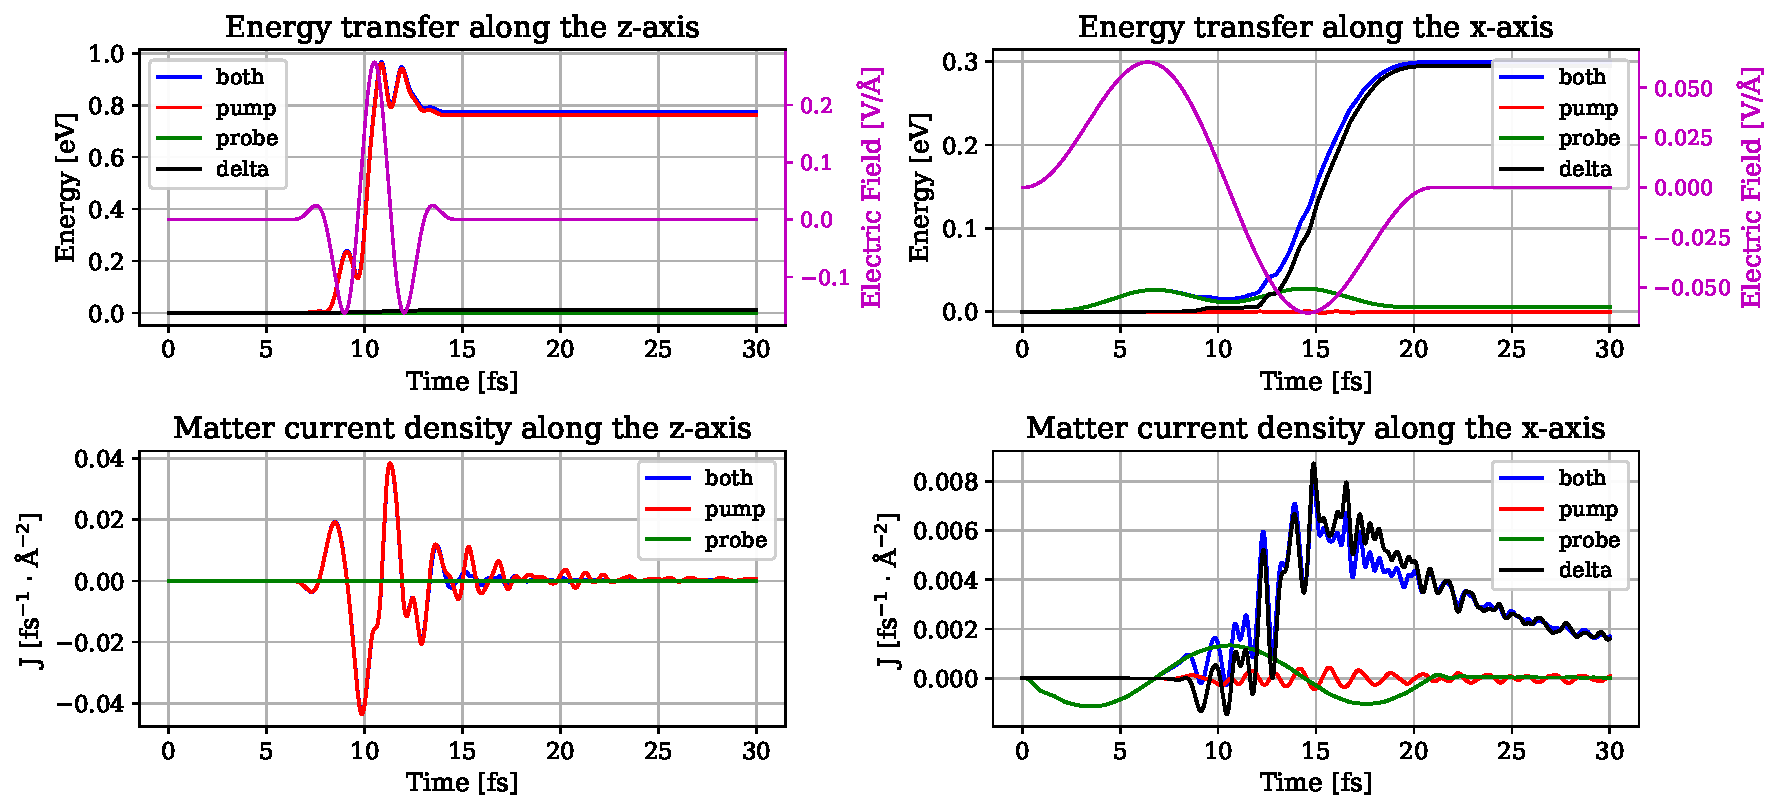
\includegraphics[width=1\linewidth]{all_pdf/additional/5_energy_current_c333_amorphous_0_92_s0_050_r18_k16_a1_i804_t9_p4d10.pdf}
    \caption{Example of pump-probe dynamics for 0.05 displacement disorder.}
    \label{fig:pp_example}
\end{figure}

Figure~\ref{fig:pp_example} illustrates the pump--probe protocol and the decomposition of responses. In the legend, ``both'' denotes the simultaneous presence of the two pulses; ``pump'' denotes the pump-only response and ``probe'' denotes the probe-only response. We analyze energy transfer and matter current density along both polarization axes. The probe pulse is weak in the sense that its direct contribution to energy absorption during pumping is small; nevertheless, it measurably affects the pump-induced dynamics along $z$. A natural interpretation is that the orthogonal field perturbs the phase coherence of the interband polarization created by the pump, thereby modifying how efficiently the pump builds up coherent oscillators. Related pump--probe-induced modifications of coherence and band-structure response have been discussed in attosecond experiments in silicon \cite{Schultze2014Si}.

Along the $x$-axis, the energy transfer remains negligible for small disorder, yet the probe-induced current can be large because it mainly reflects intraband acceleration. Therefore, to isolate transport of photoinjected carriers we analyze the current difference
\begin{equation}
\Delta J_x(t) = J_{\mathrm{both}}(t) - J_{\mathrm{pump}}(t) - J_{\mathrm{probe}}(t).
\label{eq:deltaJ}
\end{equation}
Subtracting the pump-only contribution is also essential because in a single finite supercell, local anisotropy can produce a small spurious orthogonal current. In a macroscopic disordered medium, or after sufficient ensemble averaging over disorder realizations, this term vanishes by symmetry.

\begin{figure}[h!]
    \centering
    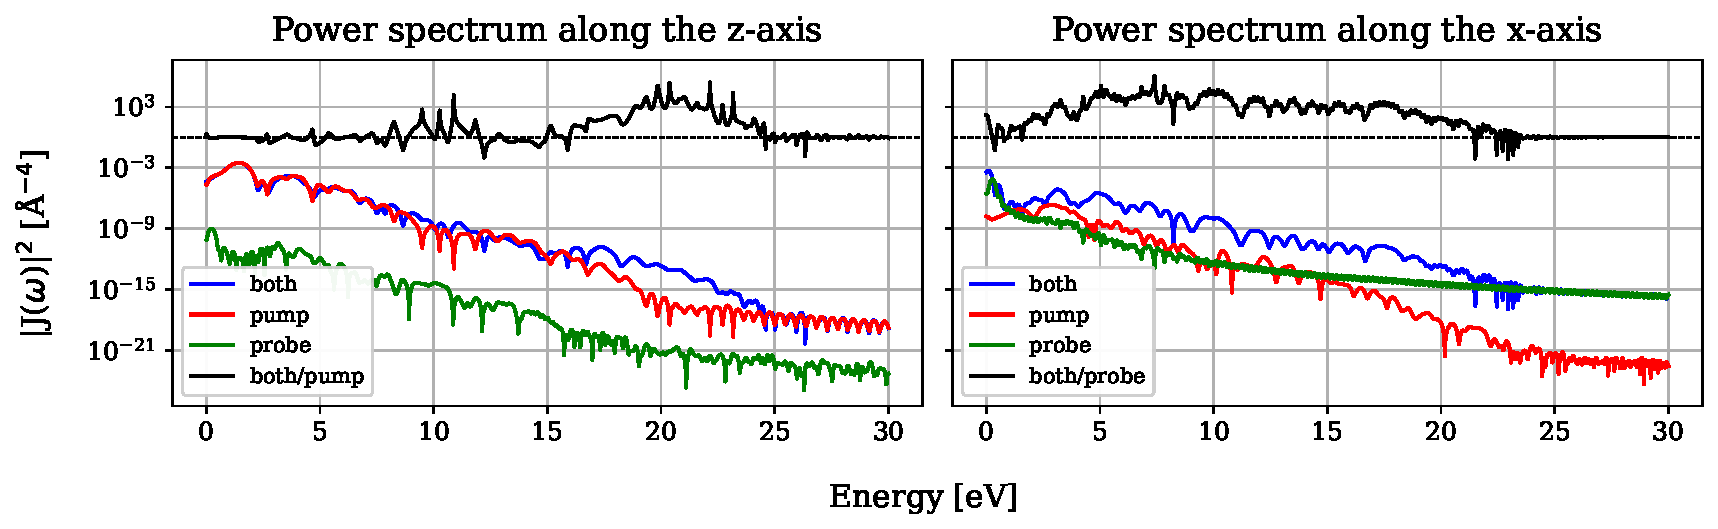
\includegraphics[width=1\linewidth]{all_pdf/additional/5_hhg_amorphous_0_92_s0_050_r18_k16_a1_i804_t9_p4d10_1d12.pdf}
    \caption{Power spectrum of currents. The ratio of the currents is shown in black.}
    \label{fig:pp_psd}
\end{figure}

The corresponding current power spectra are shown in Fig.~\ref{fig:pp_psd}. Along the $z$-axis, the probe present during pumping suppresses visibly coherent oscillations in the time domain, yet can increase nonlinearity signatures in the spectrum through field mixing. Along the $x$-axis, the pump--probe configuration enhances the low-frequency spectral weight compared with the probe-only case, consistent with the appearance of a long-lived current envelope arising from intraband motion of the photoinjected carrier ensemble. The separation between interband coherence (responsible for high-frequency components) and intraband transport (responsible for low-frequency components) is naturally formulated within semiconductor Bloch frameworks \cite{Golde2008HHGsolids,Vampa2015Semiclassical}.

\section{Response to a Probe Pulse}

We now focus on $\Delta J_x(t)$ as defined in Eq.~\eqref{eq:deltaJ} and study how disorder governs the probe-driven transport of photoinjected carriers.

\begin{figure}[h!]
    \centering
    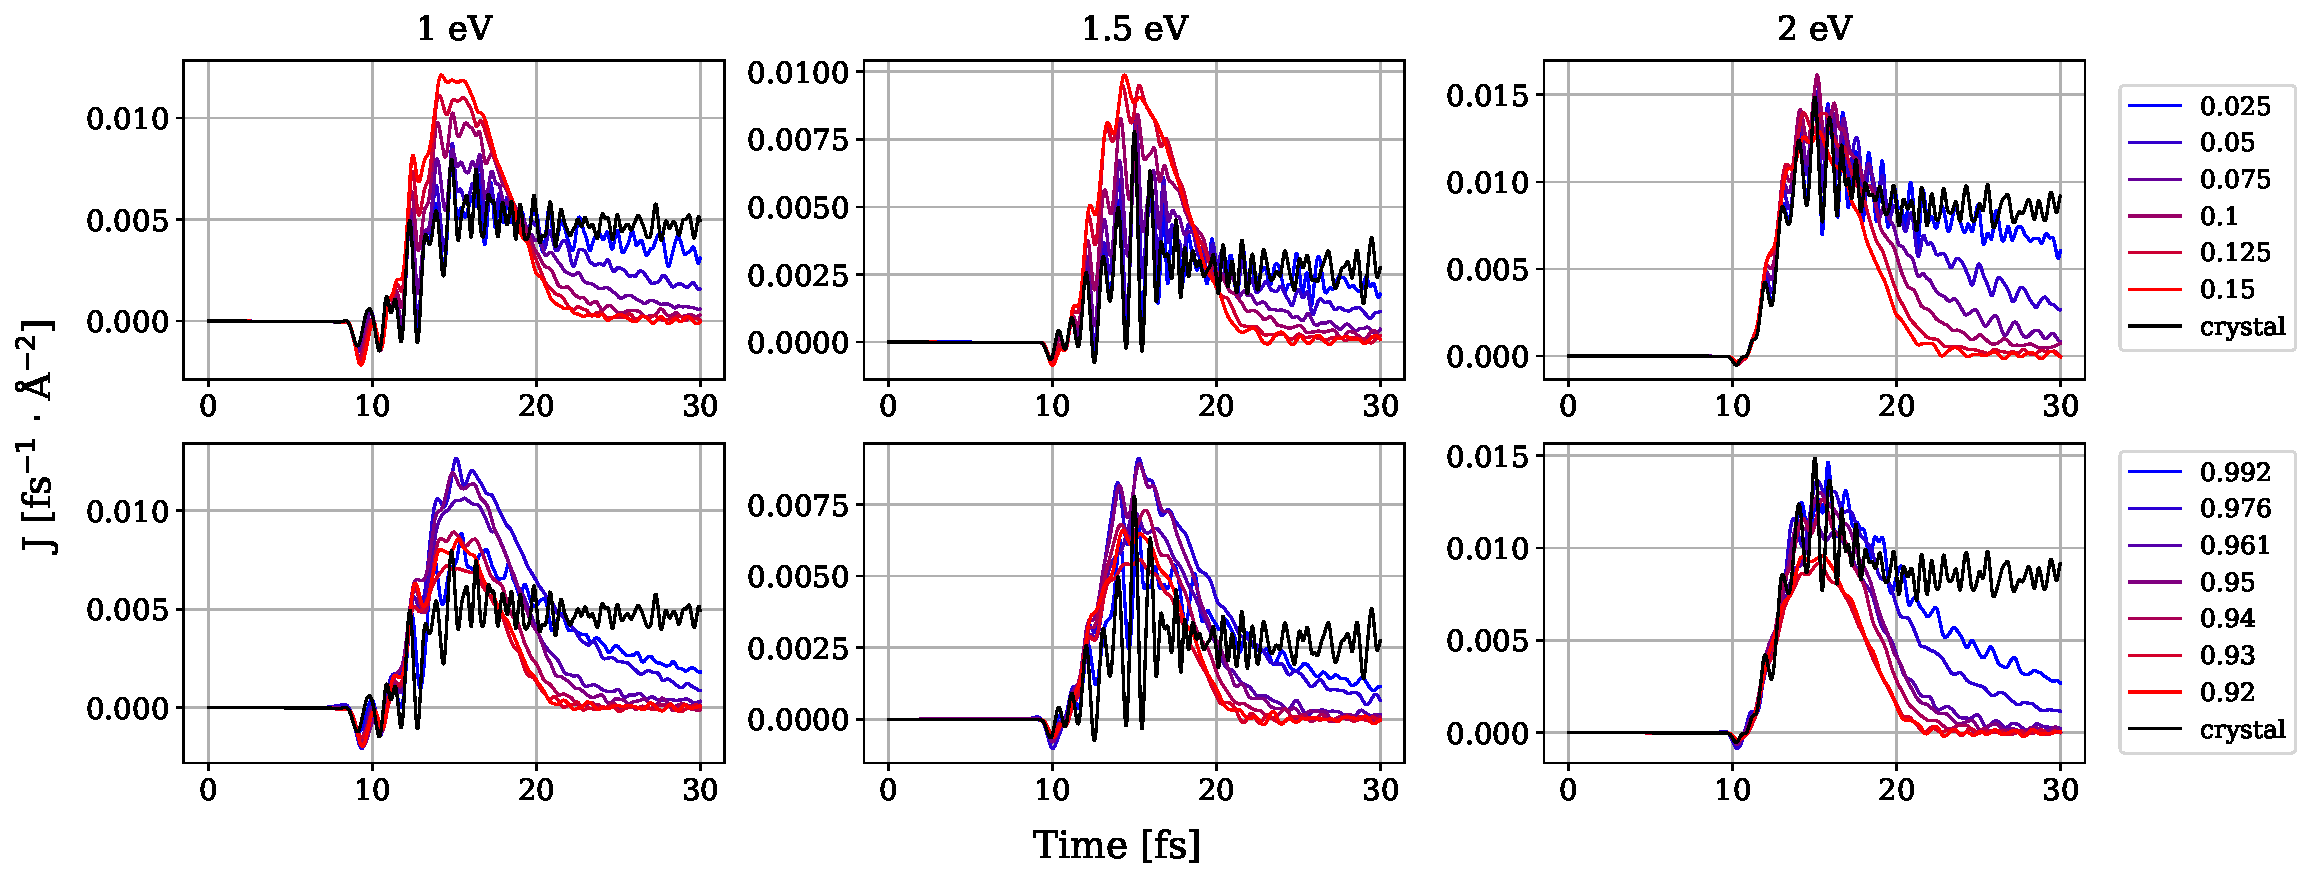
\includegraphics[width=1\linewidth]{all_pdf/drude/pdf/delta_x_current_response_comparison.pdf}
    \caption{Pump-probe current response comparison. The column caption in eV indicates the carrier frequency of the pump pulse. The top row represents displacement disorder, whereas the bottom row represents amorphous disorder.}
    \label{fig:delta_x_current}
\end{figure}

Figure~\ref{fig:delta_x_current} shows that, after photoinjection, the probe generates a substantial current response which evolves during the probe field and decays afterward. In an ideal crystal within a collisionless RT-TDDFT setting, the post-pulse current does not decay because there is no intrinsic irreversible scattering channel. With static disorder, the current envelope decays, and as shown below this decay is well described by an exponential law. Such exponential relaxation is consistent with semiclassical elastic momentum scattering in a static disorder potential treated in the Born approximation \cite{Mahan2000,AshcroftMermin}.

At the same time, the oscillatory structure sitting on top of the current envelope is suppressed with increasing disorder. These high-frequency oscillations are inherited from coherent interband dynamics excited by the pump; as disorder accelerates dephasing along $z$, the corresponding high-frequency components diminish and therefore become less visible in $\Delta J_x(t)$ as well.

Within the Drude picture, the probe-direction current obeys
\begin{equation}
\frac{dJ_x}{dt} = \frac{ne^2}{m^*(t)} E_x(t) - \frac{J_x}{\tau_m},
\label{eq:drude}
\end{equation}
where $n$ is the photoinjected carrier density, $\tau_m$ is the momentum (transport) relaxation time, and $m^*(t)$ is an effective mass that may depend on the instantaneous reciprocal-space displacement of the wave packet. The physically appropriate transport time is the momentum relaxation time, not the single-particle lifetime, and can be expressed as \cite{AshcroftMermin,Mahan2000}
\begin{equation}
\frac{1}{\tau_m(k)} = \sum_{k'} W_{k\to k'}\left(1-\cos\theta_{kk'}\right),
\label{eq:taum_def}
\end{equation}
where $W_{k\to k'}$ is the elastic scattering rate and $\theta_{kk'}$ is the scattering angle.

\begin{figure}[h!]
    \centering
    
\includegraphics[width=0.6\linewidth]{all_pdf/drude/pdf/1.5eV_12fs_sigma_0.125.pdf}
    \caption{Example of a pump-probe response.}
    \label{fig:example_pp}
\end{figure}

Figure~\ref{fig:example_pp} shows a representative pump--probe response and its envelope analysis. The tail is accurately described by an exponential function, allowing extraction of $\tau_m$. We approximate the envelope by a spline (polynomial degree 5) and evaluate its derivative in the time window relevant to the second half-cycle of the probe pulse. Once $\tau_m$ is determined, Eq.~\eqref{eq:drude} can be inverted to extract an effective mass from the measured derivative:
\begin{equation}
m^*(t) = \frac{ne^2 E_x(t)}{\frac{dJ_x}{dt} + \frac{J_x(t)}{\tau_m}}.
\label{eq:mstar_extract}
\end{equation}
This procedure reveals that, while $\tau_m$ depends primarily on disorder strength, an accurate description of the waveform requires allowing $m^*$ to vary appreciably as the wave packet is displaced in $k$-space.

\begin{figure}[h!]
    \centering
    
\includegraphics[width=0.9\linewidth]{all_pdf/drude/pdf/momentum_relaxation_time_on_wave_vector.pdf}
    \caption{Momentum relaxation time dependence on crystal momentum.}
    \label{fig:taum_k}
\end{figure}

Figure~\ref{fig:taum_k} demonstrates that the extracted transport time depends only weakly on the crystal-momentum shift induced by the probe pulse. The left panel compares two probe amplitudes corresponding to shifts of $\pi/a$ and $2\pi/a$; despite the large difference in displacement, relative standard error is of about 15\% overall. The right panel shows that, for a fixed disorder level (0.1 Å), $\tau_m$ has a relative standard error of about 7\%. This supports treating $\tau_m$ as approximately constant for a given disorder strength and attributing the main remaining waveform variability to $m^*(t)$.

\begin{figure}[h!]
    \centering
    
\includegraphics[width=0.9\linewidth]{all_pdf/cco/pdf/momentum_relaxation_time.pdf}
    \caption{Momentum relaxation time dependence on disorder strength. The legend in eV denotes the carrier frequency of the pump pulse. For displacement disorder, a fit proportional to $\sigma^{-1.5}$ is shown for comparison with the black curve, where $\sigma$ denotes the displacement variance.}
    \label{fig:taum_disorder}
\end{figure}

Figure~\ref{fig:taum_disorder} shows that $\tau_m$ decreases monotonically with increasing disorder. Remarkably, for three different average pump photon energies (corresponding to different photoinjection regimes), the extracted transport times agree within the $\sim 10\%$ uncertainty. This indicates that momentum relaxation is controlled primarily by the static disorder potential, rather than by details of how the carriers were generated.

\begin{figure}[h!]
    \centering
    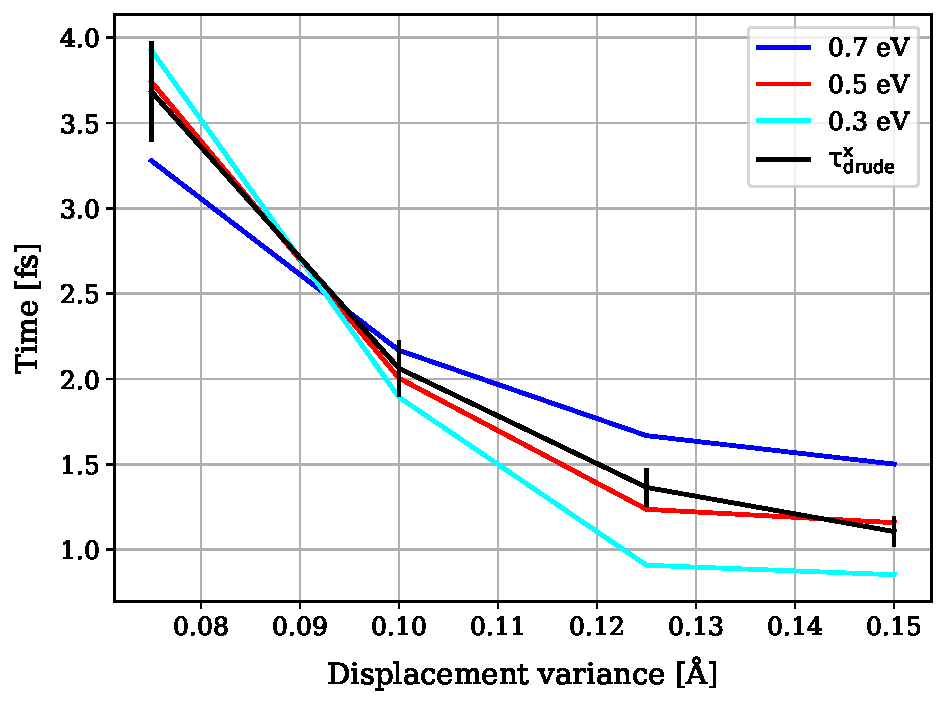
\includegraphics[width=0.7\linewidth]{all_pdf/cco/pdf/urbach_drude_comparison.pdf}
    \caption{Urbach and relaxation time comparison.}
    \label{fig:urbach_drude}
\end{figure}

Figure~\ref{fig:urbach_drude} compares $\tau_m$ to the inverse Urbach energy extracted from the DOS tail analysis by averaging the derivative on a logarithmic scale and drawing a line according to the least squares method in the energy range indicated in the graph legend from the edge of the valence band and deep into it. In disordered semiconductors, exponential band-edge tails are commonly described by the Urbach rule \cite{Urbach1953,MottDavis1979}. The observed correlation suggests that the same microscopic potential fluctuations that generate the band-edge tail also govern elastic scattering rates responsible for momentum relaxation. Although our finite-size DOS does not always provide an extended region of perfect exponential behavior, averaging the slope of $\ln g(E)$ over a controlled energy interval yields a robust proxy that tracks $\tau_m$.

\begin{figure}[h!]
    \centering
    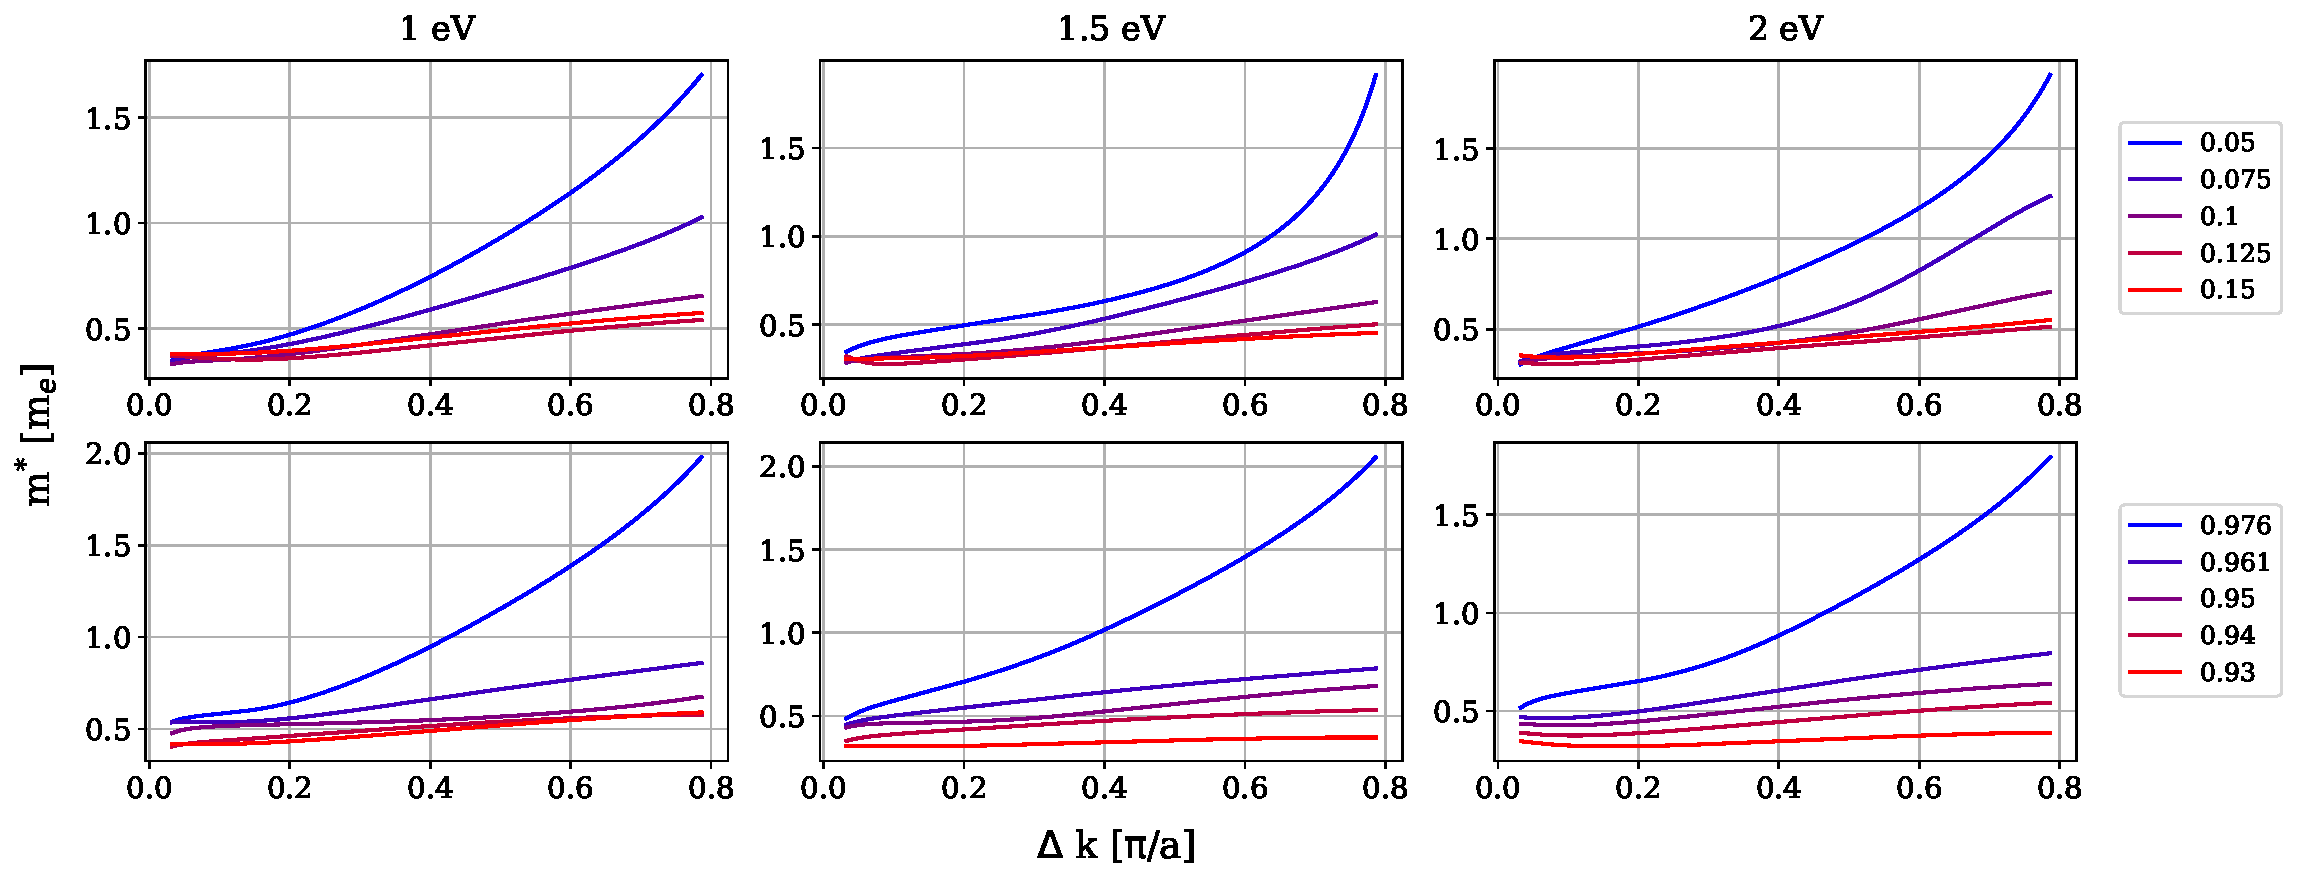
\includegraphics[width=1\linewidth]{all_pdf/drude/pdf/wave_vector_dependence_of_the_effective_mass.pdf}
    \caption{Crystal-momentum dependence of the effective mass. The column caption in eV indicates the carrier frequency of the pump pulse. The top row represents displacement disorder, whereas the bottom row represents amorphous disorder.}
    \label{fig:mstar_kdep}
\end{figure}

Figure~\ref{fig:mstar_kdep} shows the extracted effective mass as a function of crystal-momentum displacement. The key trend is that with increasing disorder the range of $m^*$ variation decreases. A consistent physical interpretation is that disorder relaxes momentum selection, enabling more uniform conduction-band population, which effectively averages over band-curvature variations and reduces the sensitivity of the wave-packet response to its instantaneous $k$-space position. Related dependence of effective mass on excitation regime and carrier distribution has been reported for ultrashort-pulse injection in solids \cite{Qasim2018}.





% We now perform a simple estimate within the effective mass approximation to evaluate the quantity at zero crystal momentum (the $\Gamma$ point) assuming an equal population of quantum states. The effective masses are taken from the NSM database \cite{Ioffe_Si}.

% For the conduction band, silicon has six equivalent $\Delta$ valleys.
% Along the $[100]$ direction, two valleys contribute with the longitudinal
% mass $m_l = 0.98\,m_e$, and four with the transverse mass
% $m_t = 0.19\,m_e$. The averaged electron effective mass is therefore

% \begin{equation}
% \frac{1}{m_e^{\mathrm{eff}}}
% =
% \frac{1}{6}
% \left(
% \frac{2}{m_l} + \frac{4}{m_t}
% \right).
% \end{equation}

% Substituting numerical values, we obtain

% \begin{equation}
% m_e^{\mathrm{eff}} \approx 0.26\,m_e.
% \end{equation}

% For the valence band, we assume equal population of heavy-hole (hh),
% light-hole (lh), and split-off (so) states. Since each subband has the
% same degeneracy, the weights are $w_{hh}=w_{lh}=w_{so}=1/3$.
% Using $m_{hh}=0.49\,m_e$, $m_{lh}=0.16\,m_e$, and $m_{so}=0.24\,m_e$,
% the averaged hole effective mass is

% \begin{equation}
% \frac{1}{m_h^{\mathrm{eff}}}
% =
% \frac{1}{3}
% \left(
% \frac{1}{m_{hh}} + \frac{1}{m_{lh}} + \frac{1}{m_{so}}
% \right),
% \end{equation}

% which gives

% \begin{equation}
% m_h^{\mathrm{eff}} \approx 0.24\,m_e.
% \end{equation}

% Finally, we define the combined averaged mass (electron + hole) using
% harmonic averaging:

% \begin{equation}
% \frac{1}{m_{\mathrm{avg}}}
% =
% \frac{1}{2}
% \left(
% \frac{1}{m_e^{\mathrm{eff}}}
% +
% \frac{1}{m_h^{\mathrm{eff}}}
% \right),
% \end{equation}

% resulting in

% \begin{equation}
% m_{\mathrm{avg}} \approx 0.25\,m_e.
% \end{equation}

% This value agrees well with the observed value upon extrapolation of the curves to zero, thereby providing indirect validation of the model.




\begin{figure}[h!]
    \centering
    
\includegraphics[width=0.7\linewidth]{all_pdf/drude/pdf/drude_validation.pdf}
    \caption{Comparison of the effective mass dependence for 12 fs and 21 fs probe pulses for different displacement disorders. The dashed(solid) line refers to the 12(21) fs pulse.}
    \label{fig:drude_validation}
\end{figure}

Finally, Fig.~\ref{fig:drude_validation} validates the proposed extraction and modeling strategy. For different disorder realizations and two probe-pulse durations (12 fs and 21 fs), the effective-mass dependence inferred from Eq.~\eqref{eq:mstar_extract} is consistent within the statistical uncertainty. The standard error is approximately 15\% for $m^*$, while the spread for $\tau_m$ is about 10\%. Since $m^*$ varies by nearly a factor of two across the explored displacement range, this level of consistency provides strong evidence that a generalized Drude description with an approximately disorder-controlled $\tau_m$ and a $k$-dependent effective mass captures the essential physics of the probe-direction current dynamics.
